\documentclass[10pt,a4paper]{article}
\usepackage[utf8]{inputenc}
\usepackage[T1]{fontenc}
\usepackage{amsmath}
\usepackage{amssymb}
\usepackage{graphicx}
\usepackage{nicematrix}
\usepackage[left=2.00cm, right=2.00cm, top=2.00cm, bottom=2.00cm]{geometry}
\usepackage{float}
\usepackage{caption}
\usepackage{subcaption}
\usepackage{multirow}
\usepackage{diagbox}
\usepackage{color}
\usepackage[
	colorlinks=true,
	linkcolor=blue,
	filecolor=blue,      
	urlcolor=cyan,
	citecolor=cyan,    
]{hyperref}
\usepackage{algorithm}
\usepackage{algpseudocode}
\usepackage{listings} % 插入代码用到
\usepackage{xcolor}
\usepackage{listings}
\usepackage{multicol}
\setcounter{tocdepth}{4}
\setcounter{secnumdepth}{4}

\definecolor{mygreen}{rgb}{0,0.6,0}
\definecolor{mygray}{rgb}{0.5,0.5,0.5}
\definecolor{mymauve}{rgb}{0.58,0,0.82}
\lstset{
 backgroundcolor=\color{lightgray}, 
 basicstyle = \footnotesize,       
 breakatwhitespace = false,        
 breaklines = true,                 
 captionpos = b,                    
 commentstyle = \color{mygreen}\bfseries,
 extendedchars = false,             
 frame =shadowbox, 
 framerule=0.5pt,
 keepspaces=true,
 keywordstyle=\color{blue}\bfseries, % keyword style
 language = C++,                     % the language of code
 otherkeywords={string}, 
 numbers=left, 
 numbersep=5pt,
 numberstyle=\tiny\color{mygray},
 rulecolor=\color{black},         
 showspaces=false,  
 showstringspaces=false, 
 showtabs=false,    
 stepnumber=1,         
 stringstyle=\color{mymauve},        % string literal style
 tabsize=2,          
 title=\lstname                      
}
\title{\textbf{CIE6107 - Robotics and Intelligent Systems \\Assignment 1}}
\author{Zixing JIANG}
\begin{document}
	
\begin{flushleft}
	CSC3180: Fundamentals of Artificial Intelligence, Spring 2023\\
	Project Report, Group 10\\
	\today
\end{flushleft}
	
\begin{flushright}\vspace{-18mm}
	
\includegraphics[height=1.7cm]{figure/logo.png}
\end{flushright}
	
\begin{center}\vspace{0.5cm}
	\textbf{\Large Adaptive Dynamic Stabilization of a Self-Balancing Scooter Using Epsilon-Greedy Q-learning}\\~\\
	\large Zixing Jiang\footnote{School of Science and Engineering, The Chinese University of Hong Kong, Shenzhen\label{SSE}}, Xuanyang Xu$^{\ref{SSE}}$, Muhan Lin$^{\ref{SSE}}$, Hongyi Yang\footnote{School of Data Science, The Chinese University of Hong Kong, Shenzhen}
\end{center}
{\noindent}\rule{\linewidth}{0.1mm}

\begin{abstract}
	In this project, we 
\end{abstract} 

\section{Introduction}
The self-balancing scooter (Figure \ref{fig:scooter}) is a common urban commuter tool. One of the most critical features in self-balancing scooter is dynamic stabilization,  which allows the scooter to maintain its balance while in motion. Without this feature, it would be very difficult for riders to stay upright and control the scooter, and even cause safety accidents in severe cases. In order to achieve dynamic stabilization, the traditional model-based automatic control methods, including Proportional-Integral-Derivative (PID) control and Model Predictive Control (MPC), model the self-balancing scooter as a cart-pole system (Figure \ref{fig:cart-pole}) and designs the controller by deriving its system dynamics. However, the dynamics-based control is sensitive to the rider's weight and center of mass (CoM) because the weight and CoM are parameters in the system's dynamics, as shown in \eqref{eq:dynamics}.

\begin{figure}[H]
	\centering
	\begin{subfigure}[b]{0.3\textwidth}
		\centering
		
\includegraphics[width=0.5\textwidth]{figure/scooter}
		\caption{Man on a self-balancing scooter}
		\label{fig:scooter}
	\end{subfigure}
	\hfill
	\begin{subfigure}[b]{0.3\textwidth}
		\centering
		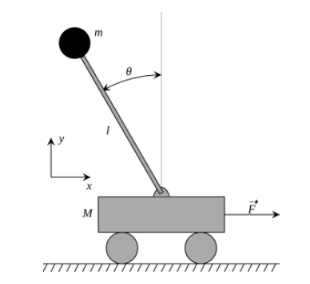
\includegraphics[width=0.85\textwidth]{figure/cart-pole}
		\caption{Cart-pole system dynamics}
		\label{fig:cart-pole}
	\end{subfigure}
	\hfill
	\begin{subfigure}[b]{0.3\textwidth}
		\centering
		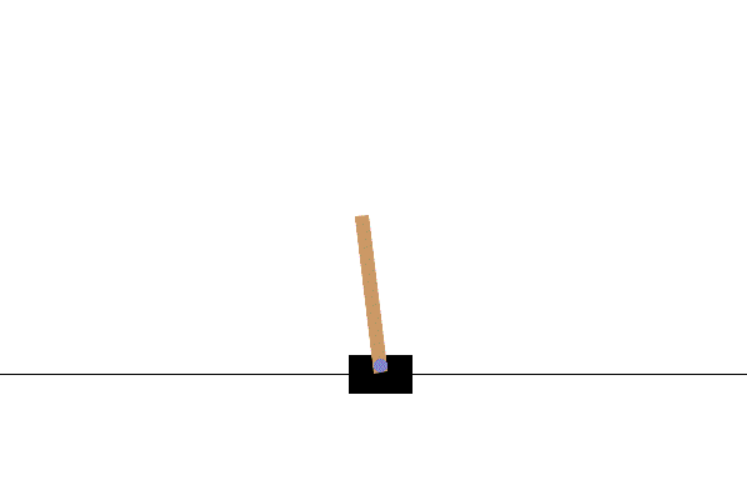
\includegraphics[width=\textwidth]{figure/open-ai}
		\caption{OpenAI Cart Pole Environment}
		\label{fig:openai}
	\end{subfigure}
	\caption{Illustrations of (a) the self-balancing scooter, (b) the cart-pole system dynamics, and (c) the OpenAI Cart Pole environment.}
	\label{fig:three graphs}
\end{figure}

\subsection*{Dynamics of the cart-pole system}
\begin{subequations}
\label{eq:dynamics}
\begin{align}
&(M + m)\Ddot{x} - ml\Ddot{\theta}cos\theta + ml\dot{\theta}^2sin\theta = F \\
&l\Ddot{\theta} - gsin\theta = \Ddot{x}cos\theta
\end{align}
\end{subequations}
where
\begin{multicols}{2}
\begin{itemize}
    \item $M$: the cart mass
    \item \textcolor{red}{$m$: the pole mass}
    \item $\Ddot{x}$: the cart acceleration 
    \item \textcolor{red}{$l$: the pole length}
    \item $\theta$: the inclination degree of the pole
    \item $\dot{\theta}$: the angular velocity of the pole
    \item $\Ddot{\theta}$: the angular acceleration of the pole
    \item $F$: the force added to the cart
\end{itemize}
\end{multicols}

It can be seen that the pole mass \textcolor{red}{$m$} and length \textcolor{red}{$l$} get involved in this kinematic model. It means controlling the cart-pole system in a dynamic way requires the information of pole mass and pole length. Once an unexpected change in pole mass or length occurs and these parameters become unknown, it is highly possible for the classical controlling method to fail, as shown in Figure \ref{fig:different_rider}.
Therefore, for riders of different weights and CoMs, the performance of stabilization with classic model-based control varies. 

To address this problem, in this project, we aim to utilize the learning ability of artificial intelligence to design a dynamic stabilizer that adapts to different rider weights and CoMs.


\begin{figure}
	\centering
	\begin{subfigure}[b]{1\textwidth}
		\centering
		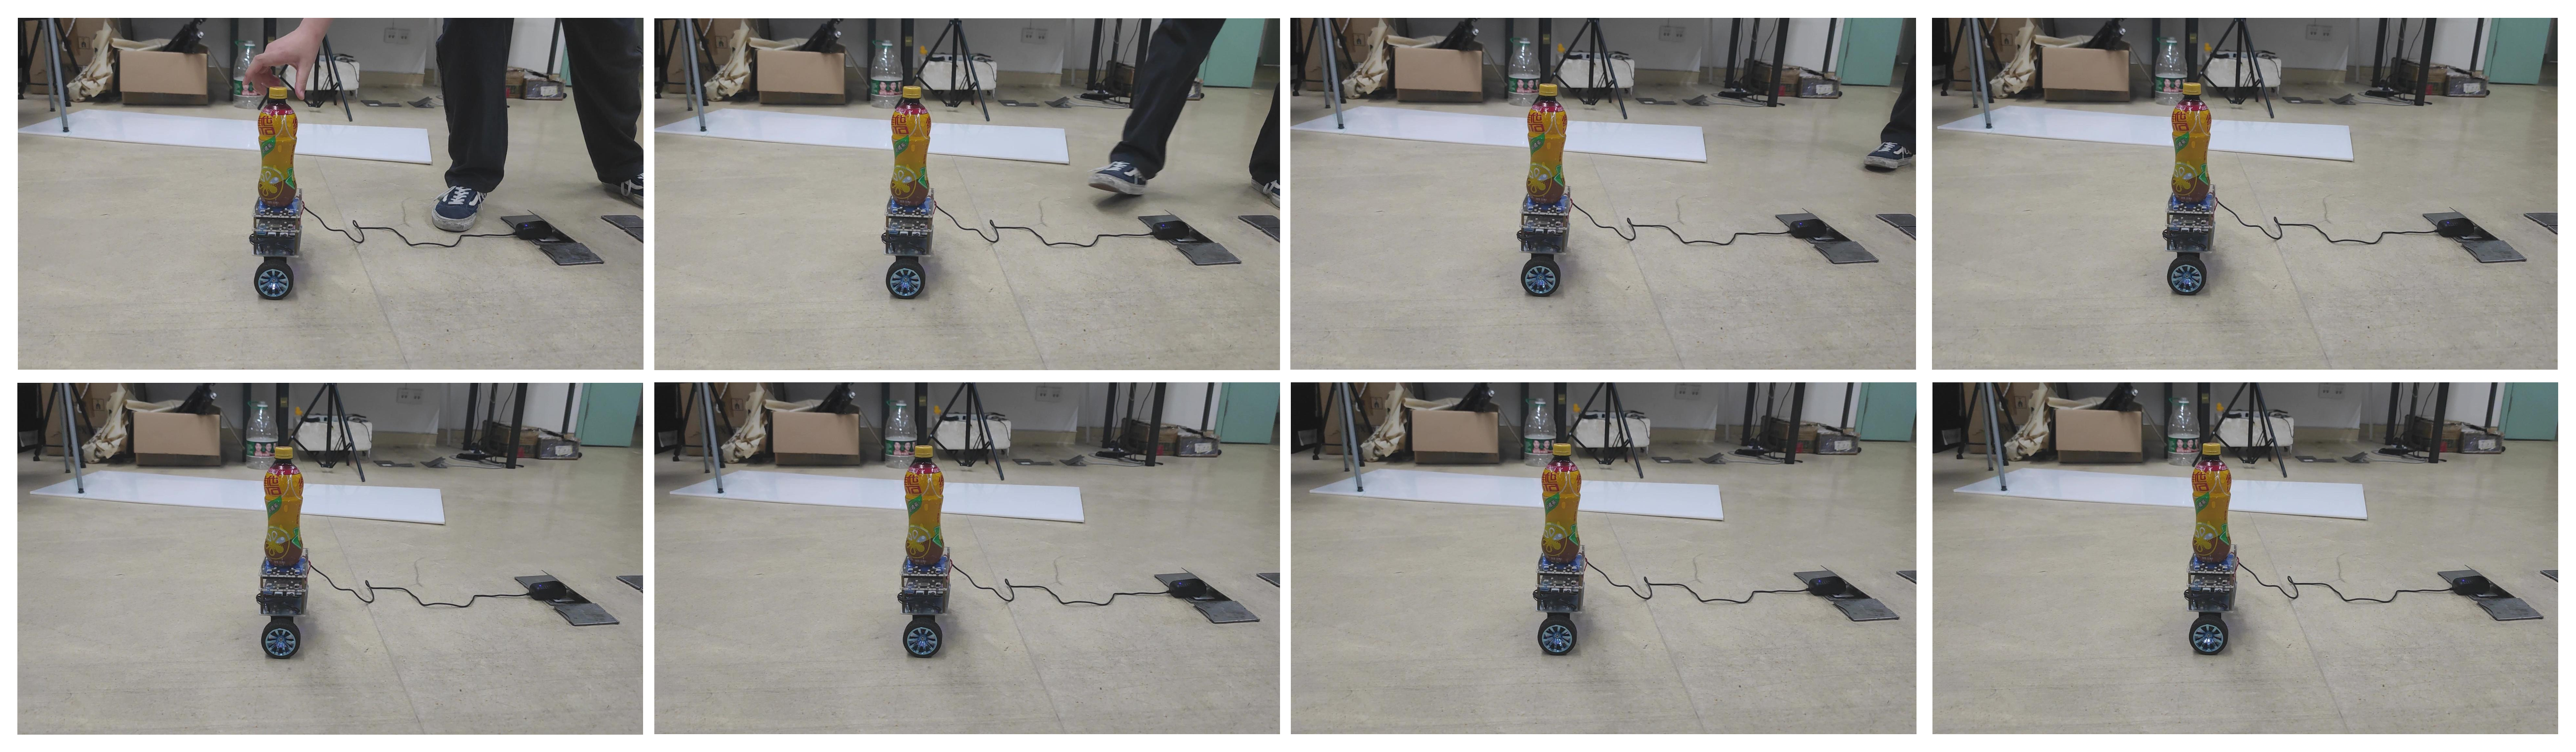
\includegraphics[width=1\linewidth]{figure/success}
		\caption{Self-balancing scooter with designed load}
		\label{fig:success}
	\end{subfigure}
	\hfill
	\begin{subfigure}[b]{1\textwidth}
		\centering
		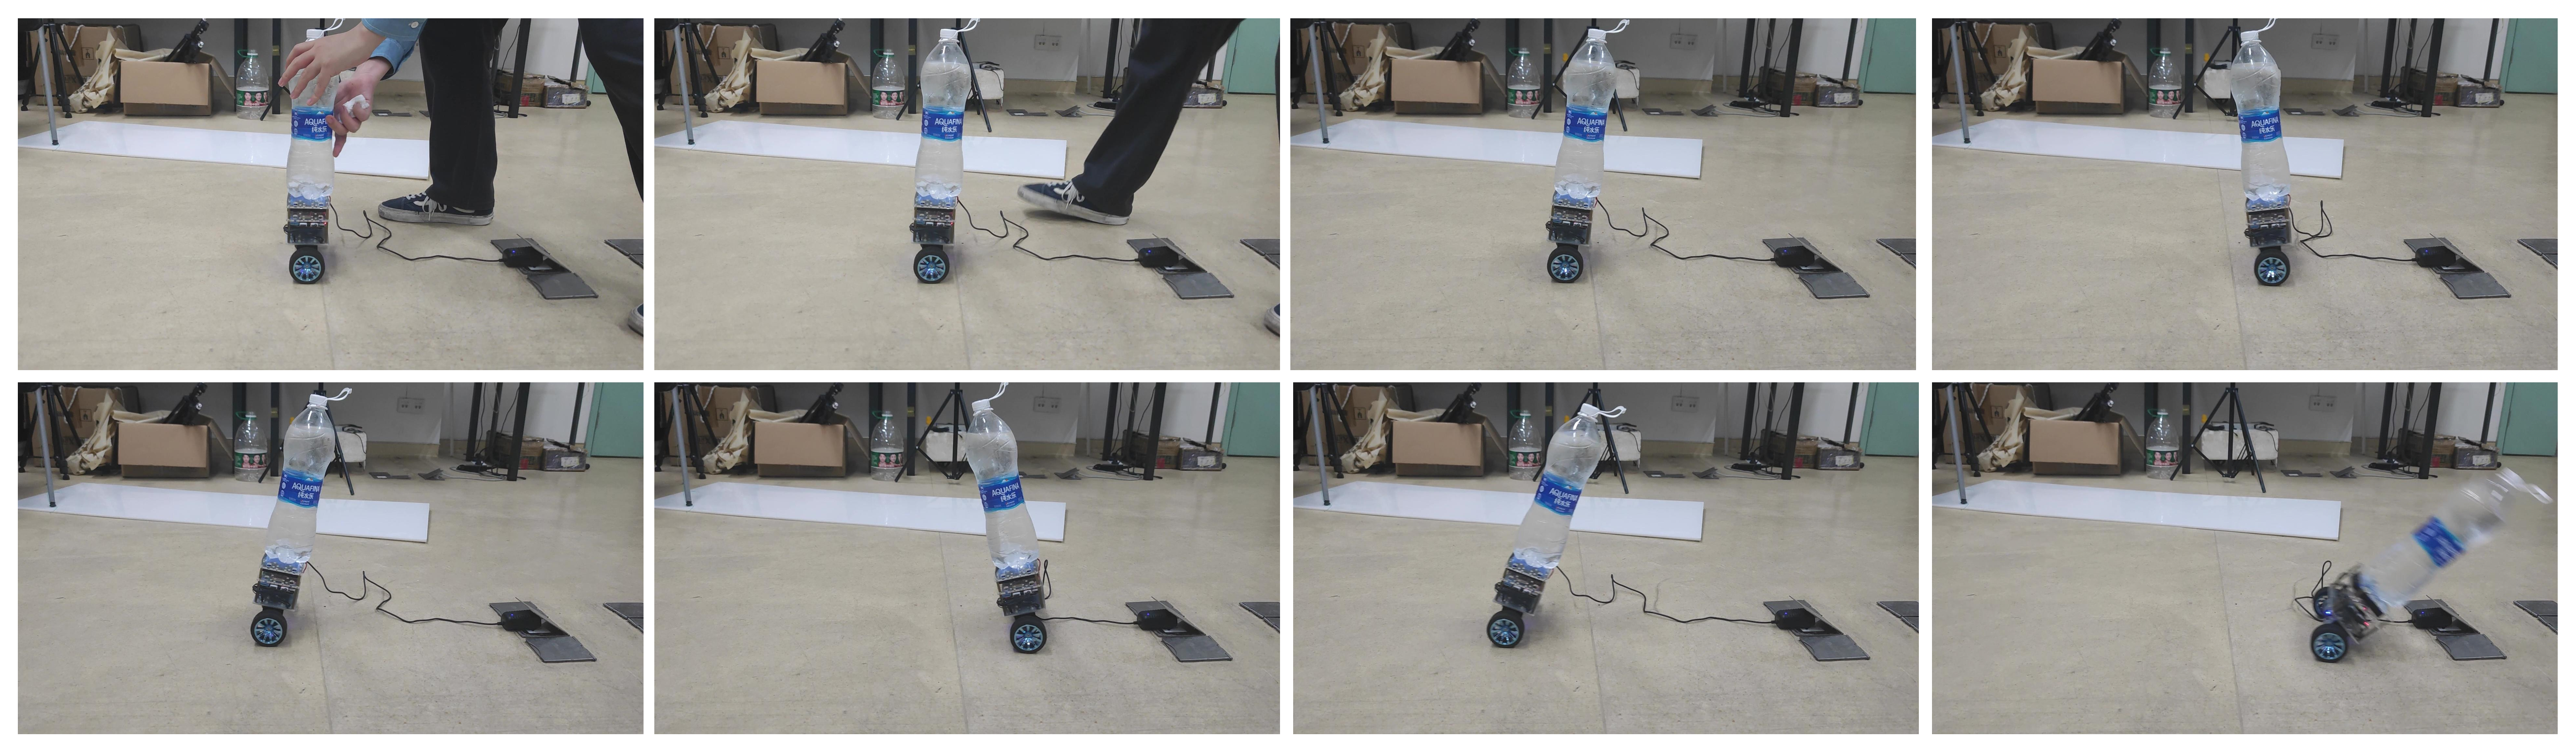
\includegraphics[width=1\linewidth]{figure/fail}
		\caption{Self-balancing scooter with a different load}
		\label{fig:fail}
	\end{subfigure}
	\caption{Model-based control is sensitive to the load's weight and CoMs. (a) The scooter succeed to maintain balance with a designed load. (b) The scooter fail to maintain balance with a different load.}
	\label{fig:different_rider}
\end{figure}

\section{Problem Statement}
In this project, we aim to solve the adaptive stabilization problem that can be stated as follows: maintain the inclination ($\theta$) of a pole with \textcolor{red}{varying mass and CoM} within a certain range by controlling the movement ($x$) of the cart (leftward or rightward).

To leverage the learning ability of artificial intelligence, we formulate the stabilization task as a reinforcement learning (RL) process. As shown in Figure \ref{fig:rl}, in each RL loop, the agent acquire an observation of state and select an action according to its understanding about the environment. The environment sends a reward to  the agent for the agent's choice, and transitions to a new state based on the agent's action and the environment's inner mechanism. In this project, the RL elements are defined as:

\begin{itemize}
	\item Agent: The cart
	\item Environment: The cart-pole system
	\item Task: Balance a length-varying pole
	\item State: A four-dimensional vector $\boldsymbol{s} = (\theta, \dot{\theta}, x, \dot{x})$
	\item Action: Direction of a fixed force exert on the cart. $\boldsymbol{a} = \left\{ left, right\right\}$
	\item Reward: An integer. If the pole does not fall down from the cart in one iteration, the sum of reward + 1. 
\end{itemize}



 
\begin{figure}
\centering
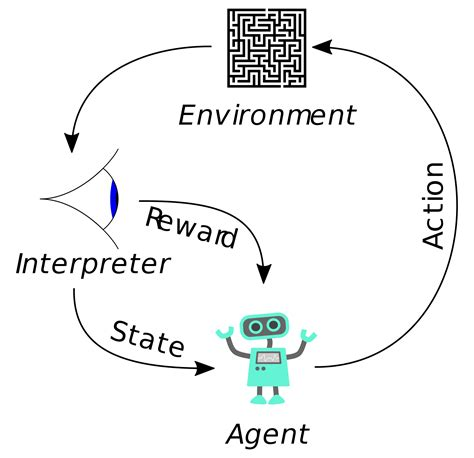
\includegraphics[width=0.3\linewidth]{figure/rl}
\caption{Framework of reinforcement learning}
\label{fig:rl}
\end{figure}



%\subsection{Reinforcement Learning}
%
%It can be seen that the pole mass and length get involved in this kinematic model. It means controlling the cart-pole system in a kinematic way requires the information of pole mass and pole length. Once an unexpected change in pole mass or length occurs and these parameters become unknown, it is highly possible for the classical controlling method to fail. It is the reason why classical model-based controlling methods perform poorly in balancing scooters with different riders.
%
%Therefore, we intend to apply reinforcement learning (RL) to solve this problem, which can adapt to the volatile cart-pole system. Namely, given the observation of the environment ($\theta, \dot{\theta}, x, \dot{x}$), we want our agent (cart) to learn a policy (move leftward or move rightward) to stable the varying pole through trail and reward. We plan to implement our RL algorithm based on the \href{https://gymnasium.farama.org/environments/classic_control/cart_pole/}{OpenAI Gym environment for cart-pole} (Figure \ref{fig:openai}). 

\section{Methodology: Epsilon-Greedy Q-Learning}
In this project, we solve the formulated reinforcement learning problem with Epsilon-Greedy Q-Learning, which is a well-developed reinforcement learning algorithm that balances exploration and exploitation in sequential decision-making problems. In this section, we will introduce the Epsilon-Greedy Q-Learning algorithm in detail and explain how we link this algorithm to the dynamic balancing problem we aim to solve. 

\subsection{Q-Learning}
Q-Learning is a classic value-based reinforcement learning algorithm that allow an agent to learn from its own actions and rewards in an environment. Unlike some other model-based control and reinforcement learning methods, it does not require a model of the environment. This feature helps to solve the traditional model-based control method's dependence on the rider's center of gravity mentioned in previous sections. 

The goal of Q-Learning is to find an optimal policy that maximizes the expected value of the total reward over any sequence of actions. The main idea of Q-Learning is to use a table, called Q-Table, that stores the estimated value $Q(\boldsymbol{s}, \boldsymbol{a})$ (Q-Value) of each action $\boldsymbol{a}$ in each state $\boldsymbol{s}$, as shown in Table \ref{tab:q-table}. The Q-Value, which reflects the value of taking a certain action in a certain state, is defined as the expectation of overall received rewards after taking action $\boldsymbol{a}$ at state $\boldsymbol{s}$, as shown in \eqref{eq:q-value}. 
\begin{equation}
	Q(\boldsymbol{s}, \boldsymbol{a}) = \mathbb{E}\left(\sum_{t = 0}^{\infty} \gamma^{t}r(\boldsymbol{s}_{t}, \boldsymbol{a}_{t}) ~\left|~ \boldsymbol{s}_{0} = \boldsymbol{s}, \boldsymbol{a}_{0} = \boldsymbol{a}\right.\right)
	\label{eq:q-value}
\end{equation}
where $r(\boldsymbol{s}_{t}, \boldsymbol{a}_{t})$ is the reward received from the environment for state-action pair $(\boldsymbol{s}_{t}, \boldsymbol{a}_{t})$ and $\gamma$ is the discount factor. 

In Q-Learning, in order to obtain the most accurate estimate of the Q-Value,  the Bellman Equation is applied to update $Q(\boldsymbol{s}, \boldsymbol{a})$ in every iteration that state-action pair $(\boldsymbol{s}, \boldsymbol{a})$ is chosen, as shown in \eqref{eq:bellman}
\begin{equation}
	\text{New~} Q(\boldsymbol{s}, \boldsymbol{a}) \leftarrow (1-\lambda)\text{Current~} Q(\boldsymbol{s}, \boldsymbol{a}) + \lambda \left[ r(\boldsymbol{s}, \boldsymbol{a}) + \gamma \max_{\boldsymbol{a'}}Q(\boldsymbol{s'}, \boldsymbol{a'})\right]
	\label{eq:bellman}
\end{equation}
where $r(\boldsymbol{s}, \boldsymbol{a})$ is the reward received in this iteration, $\boldsymbol{s'}$ is the transient state after taking $\boldsymbol{a}$ at $\boldsymbol{s}$, $\boldsymbol{a'}$ is the legal action at $\boldsymbol{s'}$, $\gamma$ is the discount factor, and $\lambda$ is the learning rate. 

In the Q-Learning process, the agent updates the Q-Table as it explores the environment and receives feedback. The agent chooses the action $\boldsymbol{a}^{*}(\boldsymbol{s})$ that has the highest value in the current state $\boldsymbol{s}$, according to the Q-Table, as shown in \eqref{eq:action-selection}.  
\begin{equation}
	\boldsymbol{a}^{*}(\boldsymbol{s}) = \arg\max_{\boldsymbol{a}}Q(\boldsymbol{s}, \boldsymbol{a})
	\label{eq:action-selection}
\end{equation}
This way, the agent learns to act optimally over time.

In our scenario, the state vector $\boldsymbol{s}$ of the cart-pole system is continuous. In order to prevent infinitely many state-action pairs, we discretized the system's state space by intervals. The length of each interval is fine-tuned to ensure the effectiveness of learning. Plus, since the Q-Table is keeping updating during the algorithm runtime, it is adaptive to dynamic environment parameters. Therefore the stabilization controller built with Q-Learning is capable of adapting to varying rider weights and CoMs.

\begin{table}
\centering
\begin{tabular}{|c|c|c|c|c|}
\hline
\diagbox{States}{Actions}& $\boldsymbol{a}_{0}$ & $\boldsymbol{a}_{1}$ & $\boldsymbol{a}_{2}$ & \dots \\
\hline
$\boldsymbol{s}_{0}$ & $Q(\boldsymbol{s}_{0}, \boldsymbol{a}_{0})$ & $Q(\boldsymbol{s}_{0}, \boldsymbol{a}_{1})$ & $Q(\boldsymbol{s}_{0}, \boldsymbol{a}_{2})$ & \dots \\
\hline
$\boldsymbol{s}_{1}$ & $Q(\boldsymbol{s}_{1}, \boldsymbol{a}_{0})$ & $Q(\boldsymbol{s}_{1}, \boldsymbol{a}_{1})$ & $Q(\boldsymbol{s}_{1}, \boldsymbol{a}_{2})$ & \dots \\
\hline
$\boldsymbol{s}_{2}$ &$Q(\boldsymbol{s}_{2}, \boldsymbol{a}_{0})$ & $Q(\boldsymbol{s}_{2}, \boldsymbol{a}_{1})$ & $Q(\boldsymbol{s}_{2}, \boldsymbol{a}_{2})$ & \dots \\
\hline
$\boldsymbol{s}_{3}$ & $Q(\boldsymbol{s}_{3}, \boldsymbol{a}_{0})$ & $Q(\boldsymbol{s}_{3}, \boldsymbol{a}_{1})$ & $Q(\boldsymbol{s}_{3}, \boldsymbol{a}_{2})$ & \dots \\
\hline
\dots & \dots & \dots & \dots & \dots \\
\hline
\end{tabular}
\caption{An example of Q-Table. $Q(\boldsymbol{s}_{i}, \boldsymbol{a}_{j})$ denotes the Q-Value of a state-action pair ($\boldsymbol{s}_{i}, \boldsymbol{a}_{j}$). The higher $Q(\boldsymbol{s}_{i}, \boldsymbol{a}_{j})$ is, the more worthy to take action $\boldsymbol{a}_{j}$ at state $\boldsymbol{s}_{i}$. } 
\label{tab:q-table}
\end{table}

\subsection{Epsilon-Greedy Action Selection}
In order to learn an optimal Q-table, we want our algorithm to explore all possible state-action pairs. Thus, in addition to the action selection criterion \eqref{eq:action-selection},  an epsilon-greedy policy is applied. Given an epsilon-greedy factor $0 \le \varepsilon \le 1$, in each iteration, there is a probability of $\varepsilon$ that the agent takes random actions to explore new possible state-action pairs, and there is a probability of $1 - \varepsilon$ that the agent exploits investigated state-action pairs via the Q-Table. The overall logic flow of the Epsilon-Greedy Q-Learning is shown in algorithm \ref{alg:egql}. 

\begin{algorithm}
\caption{Epsilon-Greedy Q-Learning}\label{alg:egql}
\begin{algorithmic}
\Require observation of state $\boldsymbol{s}$, epsilon-greedy factor $\varepsilon \in [0,1]$
\While{learning not terminate}
\State Generate a random number $i \in [0,1]$
\If{$i \le \varepsilon$}
\State Take random action $\boldsymbol{a}$
\Else
\State Select action $\boldsymbol{a}$ according to the Q-Table \Comment{Equation \eqref{eq:action-selection}}
\EndIf
\State Update Q-Table entry for $(\boldsymbol{s}, \boldsymbol{a})$ according to the received reward $r(\boldsymbol{s}, \boldsymbol{a})$ \Comment{Equation \eqref{eq:bellman}}
\EndWhile
\end{algorithmic}
\end{algorithm}

\section{Experiments Analysis}
We implemented the proposed Epsilon-Greedy Q-Learning with Python 3.11 and tested it in a modified OpenAI Gym "cart-pole" environment, which will be introduced in section \ref{5.2}. 



\section{Resources}
Here we list  the resources that we used to complete the project. 

\subsection{Project Repository}
All files of this project are hosted on a public repository \href{https://github.com/zixingjiang/CSC3180-Cart-Pole}{CSC3180-Cart-Pole} on GitHub. 


\subsection{Modified "cart-pole" Environment}\label{5.2}
In this project, we customized the OpenAI Gym environment for the cart-pole problem to create a more challenging scenario for our RL agent. We adjusted the cart's mass, pole length, and gravitational constant to create a more volatile environment that our agent could learn to balance the pole in. The customized environment is "csc3180\_cartpole\_env". You can find the source code at "CSC3180-Cart-Pole/src/csc3180\_cartpole\_env".

Our aim was to train an agent using an RL algorithm that could maintain balance for as long as possible in this customized environment. As part of our project, we customized the environment and designed specific APIs for the RL simulation program, such as "change\_poleLength", "change\_poleMass" and "set\_i\_episode". These APIs allowed the RL simulation program could effectively train the agent in the customized environment and improve performance in the specific task we designed. 

\subsubsection{How to run our code with the customized Environment}
\paragraph{Create a Virtual-Env}

We highly recommend you create a virtual environment to test our project. The Virtual environment will isolate project dependencies and package installations, allowing for effective version control of packages and avoiding conflicts with other Python projects or the system environment. However, the virtual environment is not mandatory and you can skip it.

We recommend you to install the packet in the virtual env

\begin{lstlisting}[caption={Installation of virtualenv}]
pip install virtualenv virtualenvwrapper
\end{lstlisting}

Then, you first need to add some lines to your "~/.bashrc" profile. Open the file using nano , vim , or emacs and append these lines to the end:

\begin{lstlisting}[caption={Setup of Environment Path}]
export WORKON_HOME=$HOME/.local/bin/.virtualenvs
export VIRTUALENVWRAPPER_PYTHON=/usr/bin/python3
export VIRTUALENVWRAPPER_VIRTUALENV=$HOME/.local/bin/virtualenv
source $HOME/.local/bin/virtualenvwrapper.sh
\end{lstlisting}

Save the file. Then “source it” in your terminal:

\begin{lstlisting}[caption={Setup of Environment Path}]
source ~/.bashrc
\end{lstlisting}

Create a Python 3 virtual environment for csc3180

\begin{lstlisting}[caption={Create a Virtual-Env}]
mkvirtualenv csc3180 -p python3

workon csc3180
\end{lstlisting}


\paragraph{Installation by setup.py}

You can install our customized packet into your virtual environment by executing setup.py

\begin{lstlisting}[caption={To use setup.py to install our env packet}]
cd ./CSC3180-Cart-Pole/src/csc3180_cartpole_env

python3 -m pip install .
\end{lstlisting}

Once the installation process is complete, ensure that the customized environment has been installed successfully by using the "pip list" command. This will provide a comprehensive list of all installed Python packages, including  "csc3180\_cartpole\_env".


\paragraph{Run our Q-Leaning Program}
You can use the API from our customized gym environment in your Python code as below:
\begin{lstlisting}[caption={use the customized environment in python}]
import csc3180_cartpole_env
import gymnasium as gym

env = gym.make('csc3180/CartPole_v1', render_mode='human')
\end{lstlisting}

Moreover, we have successfully developed an RL algorithm that is tailored to our specific gym environment. To run the algorithm, please execute the following code, which will enable our algorithm to interact with the customized environment and begin the training process.

\begin{lstlisting}[caption={To use setup.py to install our env packet}]
cd ./CSC3180-Cart-Pole/src

python qlearning.py
\end{lstlisting}
\subsection{Project Videos}


\section{Group Information}
\begin{table}[H]
\centering
\begin{tabular}{|c|c|c|}
\hline
\textbf{Student Name} & \textbf{Student ID} & \textbf{Email}\\ 
\hline
Zixing Jiang & 119010130 & 119010130@link.cuhk.edu.cn\\ 
\hline
Xuanyang Xu & 119010361 & 119010361@link.cuhk.edu.cn\\  
\hline
Muhan Lin & 119010177 & 119010177@link.cuhk.edu.cn\\ 
\hline
Hongyi Yang & 119010379 & 119010379@link.cuhk.edu.cn\\ 
\hline
\end{tabular}
\caption{Group Information} 
\label{tab:group}
\end{table}
%\begin{itemize}
%	\item Zixing Jiang: Student ID \textcolor{blue}{119010130}, Email \textcolor{blue}{119010130@link.cuhk.edu.cn}
%	\item Xuanyang Xu: Student ID \textcolor{blue}{119010361}, Email \textcolor{blue}{119010361@link.cuhk.edu.cn}
%	\item Muhan Lin: Student ID \textcolor{blue}{119010177}, Email \textcolor{blue}{119010177@link.cuhk.edu.cn}
%	\item Hongyi Yang: Student ID \textcolor{blue}{119010379}, Email \textcolor{blue}{119010379@link.cuhk.edu.cn}
%\end{itemize}
\subsection*{Declaration of Contributions}
\begin{itemize}
	\item \textit{Project topic and proposal:} Zixing Jiang, Xuanyang Xu, Muhan Lin, Hongyi Yang
	\item \textit{Reinforcement learning environment:} Xuanyang Xu, Muhan Lin
	\item \textit{Epsilon-Greedy Q-Learning algorithm:} Zixing Jiang
	\item \textit{Experiments:} Zixing Jiang, Xuanyang Xu
	\item \textit{Project presentation video:} Hongyi Yang
	\item \textit{Project report:} Zixing Jiang, Xuanyang Xu, Muhan Lin
\end{itemize}
\end{document}